\documentclass[10pt, a4paper, onesided]{article}

\usepackage{graphicx}
\usepackage{enumitem}
%\usepackage{abstract}
%\renewcommand{\abstractname}{}    % clear the title
%\renewcommand{\absnamepos}{empty} % originally center
\renewcommand{\familydefault}{\sfdefault}
\usepackage[colorlinks=false]{hyperref}

\setlength{\parskip}{6pt}
\setlength{\parindent}{0pt}

%opening
\title{Documentation for the clickyBoard}
\author{}
\date{}

\begin{document}
\maketitle
\vspace{-40pt}

Download this document at \href{https://github.com/SecretImbecile/clickyBoard}{github.com/SecretImbecile/clickyBoard}
\tableofcontents

\section{The clickyBoard}

	The \textit{clickyBoard} is an add-on board for the Raspberry Pi computer (model B+ or later), which adds a simple switch and LED circuit for use in GPIO programming.
	
	The clickyBoard has been designed to use Cherry MX series switches or compatible switches from other manufacturers, a popular keyswitch designed for use in keyboards that are widely available and cheaply purchased.
	
	The board, through the Raspberry PI GPIO, provides four push-buttons inputs, as well as a single output through which you can control the four backlight LEDs under each key.
	
	In addition to technical documentation, this document also includes a parts list and assembly guide, for users wishing to assemble their own clickyBoard from scratch, or kit form.

\newpage
\section{Parts Required}

	\subsection{LED and Resistor choice}
	\label{LEDresistors}
	
	
	
	%\subsection{Bill of Materials}

\section{Assembly Guide}

	\subsection*{Soldering Basics}
		This guide will assume that the reader is familiar with basic soldering techniques. The components on the clickyBoard are all through-hole components, so it may be a suitable board for a novice solderer. Be aware that the 40-pin GPIO header can be tricky, especially with an old soldering iron, or thick gauge solder wire.
		
		With that said, here are some resources for learning to solder. Video tutorials are well suited for soldering, as you'll need to be able to identify a good solder joint from a bad one.
		\begin{itemize}[nolistsep]
			\item \textit{Soldering basics and choosing a cheap soldering iron} (00:00--12:00), bigclivedotcom --- \url{https://www.youtube.com/watch?v=aIab66EgfHM}
			\item \textit{EEVblog \#183 - Soldering Tutorial Part 2}, EEVblog --- \url{https://www.youtube.com/watch?v=fYz5nIHH0iY}
		\end{itemize}
	
	\subsection*{Resistors}
	
		For convenience, we always solder components from lowest height to highest, to maintain a steady PCB on which to work. Begin by soldering the two $1 k\Omega$ resistors in slots \texttt{r1} and \texttt{r2}.
		
		Next, solder the resistors for the LED array that you chose in \autoref{LEDresistors} into the sockets \texttt{r3}--\texttt{r6}. If you are using two resistors, ensure the circuit is completed1 in accordance to \autoref*{fig:documentation}.
		
		\begin{figure}[h]
			\centering
			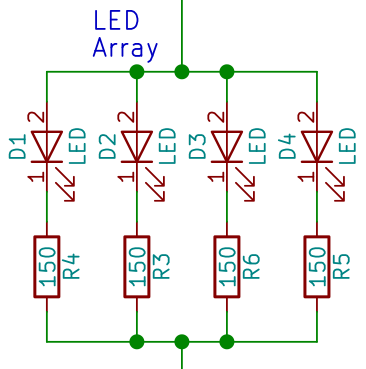
\includegraphics[width=0.25\linewidth]{img/resistor}
			\caption{Wiring schematic for the four resistor sockets}
			\label{fig:documentation}
		\end{figure}
	
	\subsection*{MOSFET}
	
		Bend the legs of your TO-220 package MOSFET to a 90 degree angle and place it in the socket so that the large metal tab is flush with the PCB, then solder the three pins. You can optionally solder the tab to the plated mounting hole.
		
		If you are \textbf{not} using a MOSFET to control the LEDs, you should jumper the two outermost pins with a piece of insulated wire or an $\approx0 \Omega$ resistor. Ensure that the jumper wire does not short with the centre contact pad.
	
	\subsection*{Switches \& LEDs}
	
		\subsubsection*{Erratum: LED pad direction}
		\label{LEDerror}
		
			Please note that the solder pads for the LEDs are reversed. By convention, the square solder pad indicates the positive side of a diode. However, because of an update to the \textit{KiCad} software, the pins in the component library were reversed. You should therefore solder the (longer) \textbf{positive} lead of the LEDs into the \textbf{circular} pads.
			
			\begin{quote}
				\textit{...all diodes in KiCad's standard libraries have seen their pin numbers swapped. This is to be in line with most other software and the IPC standard as well, which states that cathode should be pin 1.}\footnote{\url{https://forum.kicad.info/t/important-announcement-diode-pins-swapped-in-standard-kicad-libraries/820}}
			\end{quote}
	
		\subsubsection*{Switch assembly}
	
			In MX style switches, the 3mm LED sits in a slot at the bottom of the switch, and the leads are fed through holes in the switch housing. It is recommended to place the LED in the switch, then inserting that complete assembly into the board to solder.
			
			Ensure that the polarity of the LED is correct, and the switch is sitting flush with the board with the plastic peg(s) in their respective holes, then solder the connections of both the switch and LED.
	
	\subsection*{40-pin GPIO header}
	
		To complete the \textit{clickyBoard}, solder the 40-pin female header to the board, with the female socket on the reverse side of the board.
		
		If you choose not to solder all of the pins, the following pins are required (GPIO board pinout numbering): 
		\texttt{1 4 9 11 12 13 15 16}, omitting \texttt{11} if a MOSFET was not used.



\section{Example Code}

\section{Technical Documentation}
	\subsection{Schematic design for the clickyBoard}
		\begin{center}
			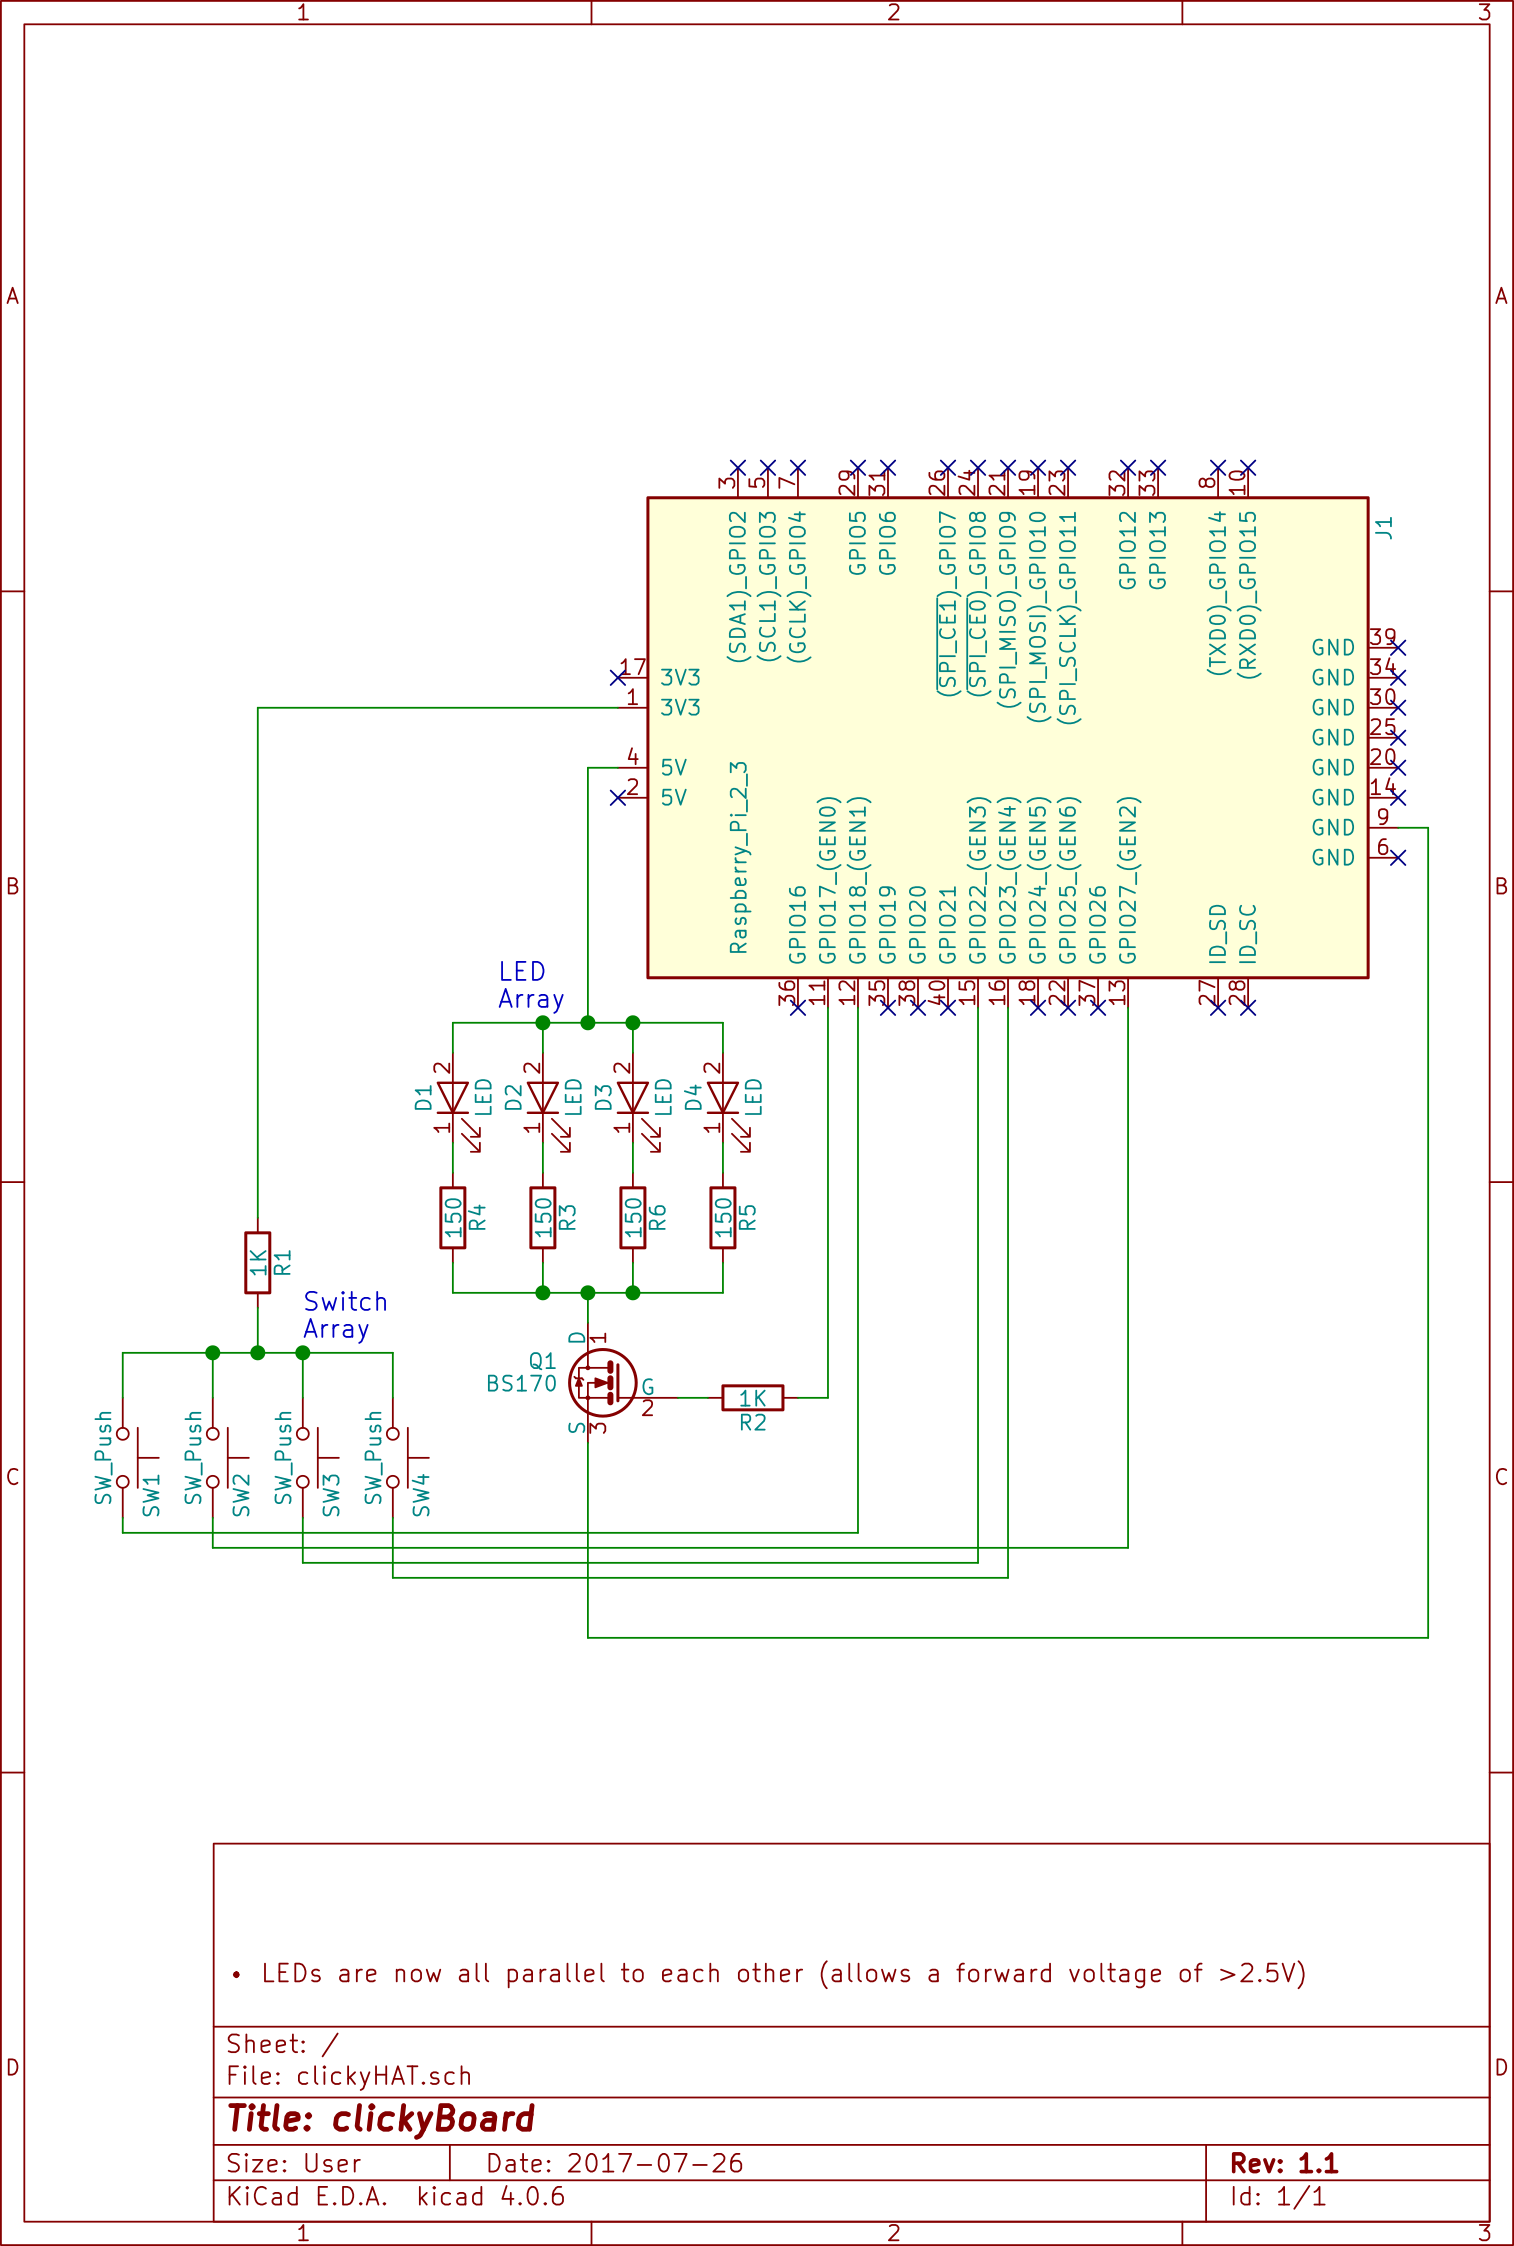
\includegraphics[width=1\linewidth]{img/schematic}
		\end{center}
	
	\newpage
	\subsection{PCB layout for the clickyBoard}
		Gerber outputs (with additional layers) are available on the \href{https://github.com/SecretImbecile/clickyBoard}{github repo}.
		\subsubsection*{Front Copper}
			\begin{center}
				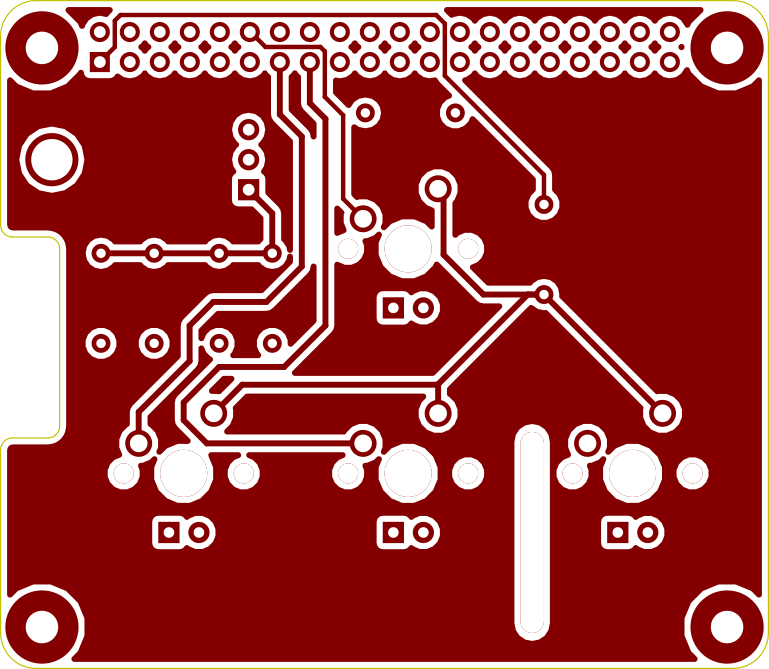
\includegraphics[width=0.7\linewidth]{img/F_Cu}
			\end{center}
		\subsubsection*{Back Copper}
		\begin{center}
			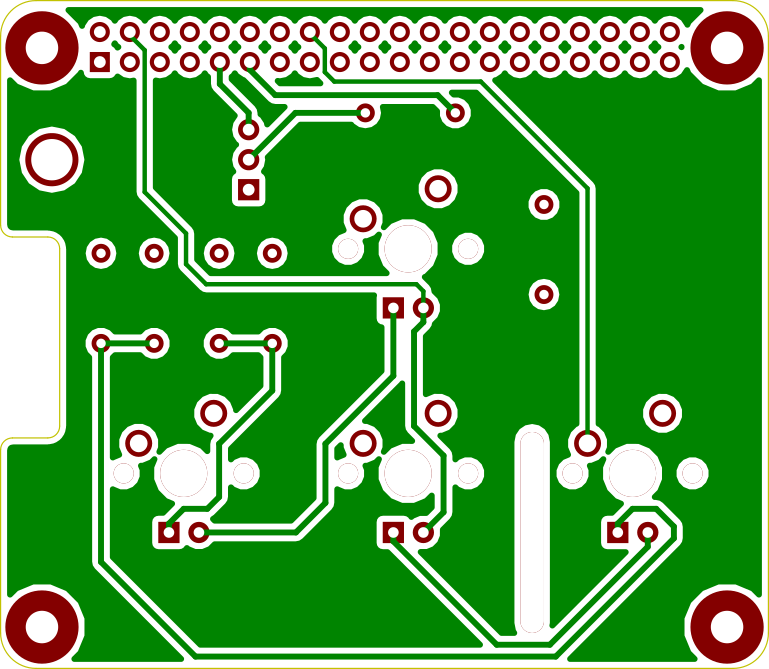
\includegraphics[width=0.7\linewidth]{img/B_Cu}
		\end{center}
		\subsubsection*{Front Silkscreen}
		\begin{center}
			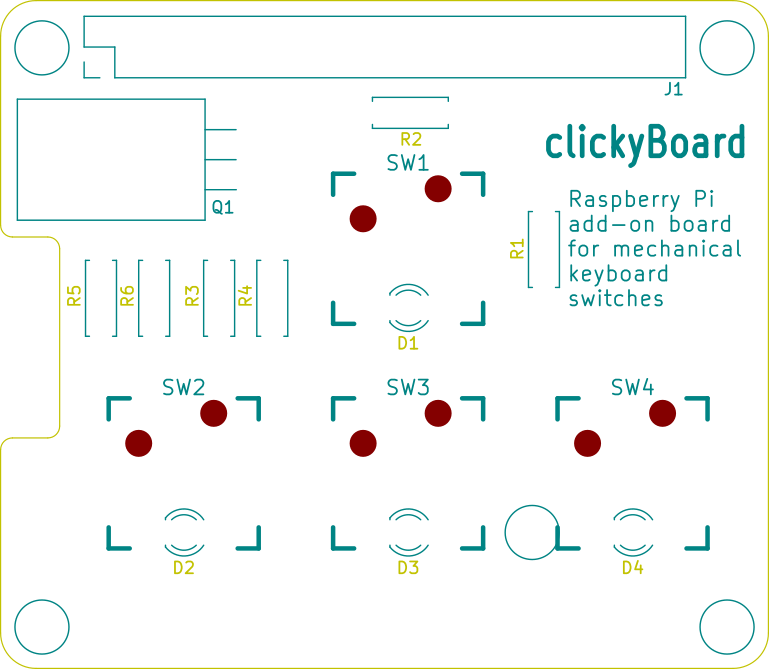
\includegraphics[width=0.7\linewidth]{img/F_Ss}
		\end{center}
	
\subsection{Design rules for PCB}

	The design rules used for this PCB were as follows.
	
	\begin{tabular}{|c|c|c|c|}
		\hline 
		Clearance & Track Width & Via Size & Silkscreen line thickness \\ 
		\hline 
		$0.2 mm$ & $> 0.375 mm$ & n/a & $> 0.15 mm$ \\ 
		\hline 
	\end{tabular} 
	

\end{document}
